\section{Existing Positioning Methods}
In this section, we will consider positioning algorithms, which can be used to estimate the location. The positioning algorithms can be divided into three types, namely geometry-based algorithms, positioning algorithms using scene analysis and proximity, and positioning algorithms using inertial measurements. Each of the algorithm types have their own weaknesses and strengths. Therefore, combining more than one algorithm could potentially lead to a better estimate of the location.

\subsection{Scene Analysis}\todo{RETTELSER HER.}
\label{sec:scene_analysis}
Algorithms which perform scene analysis work by first constructing fingerprints for a scene, then estimate the location by matching online measurements against the locations' fingerprints. This type of algorithms is also called location fingerprinting. Location fingerprinting consists of two phases, namely the offline phase and online phase. In the training phase or offline phase, the data, typically radio frequency data, is collected at access points for different known indoor positions, and a fingerprint is constructed for known indoor positions. During the online phase, the real time position is estimated by pattern matching the measured data with the fingerprints of the locations from the offline phase.\cite{IPS01} The following machine learning algorithms can perform location fingerprinting.

\subsubsection{LightGBM}
As LightGBM is a widely used algorithm by other competition participants at Kaggle, we will also be investigating this algorithm.
LightGBM is a variation of the \gls{gbdt} algorithm. \gls{gbdt} is an ensemble model of decision trees, which are trained in sequence. In each iteration, the \gls{gbdt} learns the parameters of the decision trees. A decision tree is a tree which consists of internal and leaf nodes. The internal nodes have a condition based on the observations or the input and contain two children nodes. One of the children nodes will be labeled true while the other is labeled false. Each leaf node is labeled with a class, and the classification will be the labeled class at the leaf node depending on which leaf node is reached within the tree\cite{AIBook}.
The LightGBM significantly outperforms other \gls{gbdt} algorithms like XGBoost and SGB in terms of computational speed and memory consumption, which is ideal for our case as the model should be made available on a mobile application/service. \cite{lightgbm} LightGBM is not widely used in \gls{ips} when relating to research in \gls{ips}. In the Kaggle competition, \cite{lgbmKaggle01} uses LightGBM and Wi-Fi \gls{rssi} measurements to achieve a public score of 8.34 meter based on the evaluation metric defined in \textbf{\autoref{sec:kaggleComp}}. The aforementioned LightGBM implementation achieves the lowest \textit{mean positioning error} for the LightGBM implementations at Kaggle.

\subsubsection{Artificial Neural Network}
Neural Networks are inspired by the neurons in the brain. The networks consist of neurons or units organised into layers. The typical neural network architecture is the \gls{ann}. This type of network consists of an input layer, an output layer, and a number of hidden layers\cite{AIBook}. 

The use of \gls{ann} in \gls{ips} has among other been investigated by \cite{ANN01}. The \gls{ann} model proposed by the paper consists of an input layer with four neurons, an output layer with two neurons, and four hidden layers. The indoor positioning system proposed by the paper only considers Wi-Fi \gls{rssi} data. As input to the model, it uses normalised Wi-Fi \gls{rssi} measurements from each of the access points. The environment in the paper consists of four access points and thus results in four input neurons. The output of the model will be the \textit{x} and \textit{y} coordinates. Furthermore, the amount of hidden layers for the model should depend on the number of input and output neurons. The performance of the model is evaluated through precision in the form of the \textit{position error}, and accuracy in the form of \textit{Mean Position Error}. The result of the ANN is that the ANN can achieve a error of less than 1 meter for 30\% of the instances, 10\% of the instances has an error more than 2 meters, and 60 \% of the instances has an error of 1-2 meter. 

\cite{ANN02} also investigates the feasibility of \gls{ann} in \gls{ips}. This method also uses Wi-Fi \gls{rssi} measurements as input data. Here, the results are summarised by the \textit{mean position error} and the training time for the \gls{ann}. The results are measured for two scenarios, one complex environment with increased interference and another environment with less interference. The \textit{mean position error} is around 0.21 meter for all configuration of \gls{ann} in the complex environment and 0.1 meter for the simple environment. 

The main challenge with \gls{ann} is to find the balance between computation time and performance as it is possible to achieve greater performance with deeper networks but this would also result in more computation time and therefore might not be ideal to implement in a mobile device.

\subsubsection{kNN}
The \textit{k}-Nearest Neighbors algorithm works by first finding \textit{k} nearest neighbors through a distance metric. After finding the \textit{k} nearest neighbor, the classification or prediction will be the majority of the neighbors. In a position estimation setting, instead of considering the majority of the neighbors, an average of the \textit{k} nearest neighbors is calculated. This average would then be the location estimate. The most commonly used distance metric in positioning is the Euclidean distance. \cite{IPS01} In the IPS context, a Weighted \textit{k}-Nearest Neighbors algorithm (WKNN) has been investigated by \cite{wknn}. In the WKNN, the \textit{k} nearest neighbors are first weighted according to some weights before averaging them. In this paper, the Manhattan distance achieves better results compared to the Euclidean distance. WKNN achieved an error of 1.07 meter for 80\% of the errors, and approximately 2 meter for all of the errors. This algorithm can also be used in real-time application.
%https://link.springer.com/article/10.1007/s11277-017-4295-z
%https://ieeexplore.ieee.org/stamp/stamp.jsp?tp=&arnumber=8054235

\subsubsection{Hidden Markov Model}
In the \gls{hmm}, the idea is to consider a series of measurements instead of a single signal measurements, which greatly improved the location estimation accuracy. This series of measurements makes it possible to keep track of a device's location over time. \gls{hmm} consists of two types of nodes, namely the observable nodes and hidden nodes. The observable nodes are denoted by the white circles in \textbf{\autoref{fig:hmm}}, while the hidden states are denoted by the shaded circles. We assume that hidden nodes or states only depends on the observable states. In the \gls{ips} context, the observable states will be the locations while the hidden states will be the signal measurements. \gls{hmm} has a transition probability distribution, and an emission probability distribution. The transition probabilities models the state at time $t$ based on time $t-1$ meaning that the history of 
\begin{figure}[h]
    \centering
    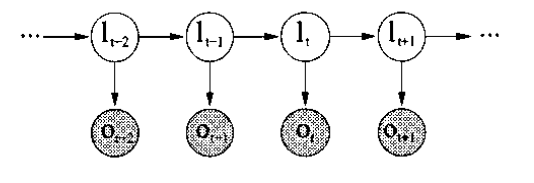
\includegraphics[scale=1.6]{Images/ProblemAnalysis/hmm_pe.PNG}
    \caption{\gls{hmm} of position tracking}
    \label{fig:hmm}
\end{figure}
% \begin{longtable}{ p{.25\textwidth}  p{.7\textwidth}}
% \textbf{Tree Based Learning} & Tree based learning employs decision tree(s) or classification tree(s) for classification. A decision tree is a tree which consists of internal and leaf nodes. The internal nodes has a condition based on the observations or the input and contains two children nodes. One of the children nodes will be labeled true while the other is labeled false. Each leaf node is labeled with a class, and the classification will be the labeled class at the leaf node depending on which leaf node is reached within the tree.\cite{AIBook}
% \\\\
% \textbf{Neural Network} & Neural Networks are inspired by the neurons in the brain. The networks consist of neurons or units organised into layers. There are many different types of neural networks, where the typical network architecture is feed-forward neural networks. This type of network consist of an input layer, an output layer, and a number of hidden layers.\cite{AIBook} 
% \\\\
% \textbf{kNN} & The \textit{k}-Nearest Neighbors algorithm works by first finding \textit{k} nearest neighbors through a distance metric. After finding the \textit{k} nearest neighbor, the classification or prediction will be the majority of the neighbors. In position estimation setting, instead of considering the majority of the neighbors, an average of the \textit{k} nearest neighbors is calculated. This average would then be the location estimate. The most commonly used distance metric in positioning is the Euclidean distance. \cite{IPS01}
% \\\\
% \textbf{Probabilistic Model} & The probabilistic model are based on Bayes' rule, and models the problem in terms of probabilities. One probabilistic method is to, given a measured signal and a number of location candidates, model the probability of each of the location candidates conditionally dependent on the measured signal. The location candidate with the highest probability would then be the location estimate.\cite{IPS02}. Other probabilistic models could also be useful in position estimation such as the Hidden Markov Model, where we in addition to the measured signal also consider the previously measured signals when estimating a position.
% \\%\\
% %\caption{presents the main recommender system types.}
% \label{table:fingerprinting}
% \end{longtable}

\subsection{Geometry Based Methods}
In this section, we will describe two different techniques to compute a position of an object geometrically.

\subsubsection{Triangulation} \label{sec:triangulation}
Triangulation is described in \cite{Triangulation}.

Triangulation is based on measuring angles of known points in space. The receiving object measures the angles towards the signals transmitted to it, known as \gls{aoa}. Different techniques are applied to measure AOA, one of the common being using an array of directionally placed sensors. Another approach is to use two sensors placed in parallel. The time point at which the sensors receive the signal is likely to be different and can be used to compute the angle of the received signal.

As seen in \textbf{\autoref{fig:AOAAngle}}, having two sensors with distance $r$ apart and distance $\Delta l$, the angle $\alpha$ can be calculated with $\alpha = \arcsin (\frac{\Delta l}{r})$, where $\Delta l$ can be represented as $\Delta t$, which can be determined by \gls{tdoa} measurement.

\begin{figure}[H]
    \centering
    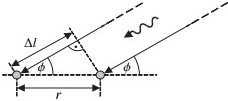
\includegraphics[scale=1.0]{Images/ProblemAnalysis/AOA_fig.jpg}
    \caption{Depiction of sensor placement to enable signal angle measurement\cite{Triangulation}.}
    \label{fig:AOAAngle}
\end{figure}

The disadvantage of triangulation is that it requires the mentioned additional sensors in order to calculate this angle.

\subsubsection{Trilateration} \label{sec:trilateration}
Trilateration is described in \cite{Triangulation}.

In trilateration, the position of an object is calculated by solving three equations of circles representing the range from the beacon to the object. This is illustrated in \textbf{\autoref{fig:trilateration}}.
By letting the beacons be denoted as $a$, $b$ and $c$, and the object to locate $m$, we can solve the following equations for $x_m$ and $ym$, where $l$ is the radius of each circle:

\begin{equation} \label{eq:CirclesCalculation1}
    (x_m - x_a)^2 + (y_m - y_a)^2 = l_{am}^2
\end{equation}
\vspace{-3mm}
\begin{equation} \label{eq:CirclesCalculation2}
    (x_m - x_b)^2 + (y_m - y_b)^2 = l_{bm}^2
\end{equation}
\vspace{-3mm}
\begin{equation} \label{eq:CirclesCalculation3}
    (x_m - x_c)^2 + (y_m - y_c)^2 = l_{cm}^2
\end{equation}

\begin{figure}[H]
    \centering
    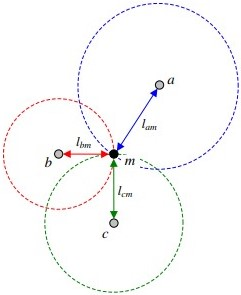
\includegraphics[scale=0.8]{Images/ProblemAnalysis/trilateration.jpg}
    \caption{Illustration of locating an object using three beacons with the use of trilateration\cite{Triangulation}.}
    \label{fig:trilateration}
\end{figure}

\subsubsection{Centroid}
How centroid location algorithms are used in locating objects is described in \cite{5759777}.

Centroid is, like triangulation and trilateration, based on beacons and the locations of the beacons. The goal is to provide a location estimate of an object given a vector of \gls{rssi} values. There exists two algorithms to locate an object: a range-based, which uses several distance to beacon estimations obtained from \gls{rss} measurements, and a range-free, which determines a location without distance estimations. These two algorithms are identified as WCL and REWL, respectively.

WCL approximates the location of an object by calculating the centroid of the coordinates of the beacons that are in range. WCL makes use of the equation seen in \textbf{\autoref{eq:WCLApproximaion}} to estimate the location of an object, where $a_i$ is the coordinates of a beacon and $\hat{d}_i$ is the distance between the object and beacon $a_i$, estimated using \gls{rss} values. Furthermore, $g > 0$ is an exponent that determines the weight of the contributions from each beacon. Using this equation, the distance from the object to each of the beacons within range is taken into account.

\begin{equation} \label{eq:WCLApproximaion}
    \hat{p} = \frac{\sum_{i = 1}^{n} (\hat{d}_i^{-g} * a_i)}{\sum_{i = 1}^{n} (\hat{d}_i^{-g})}
\end{equation}

In the estimation of the position of an object using REWL, REWL favors the beacons transmitting with higher \gls{rssi} values, since those are likely to be closer to the object. A weighting factor $\lambda$ is used in \textbf{\autoref{eq:REWLApproximation}}, where $RSS_{max}$ is the maximum value of all of the \gls{rss} measures measured by the object. The values of the weighting function $\lambda$ usually span from $0.1$ to $0.1$.

\begin{equation} \label{eq:REWLApproximation}
    \hat{p} = \frac{\sum_{i = 1}^{n} [(1 - \lambda)^{RSS_{max} - RSS_{i}} * a_i]}{\sum_{i = 1}^{n} (1 - \lambda)^{RSS_{max} - RSS_{i}}}
\end{equation}

\subsection{IMU positioning} \label{sec:IMUPositioning} % Kan måske stå et andet sted, så det kan skrives mere abstrakt her.
How positions are calculated with he use of IMU is described in \cite{IMUPositioning}.

As mentioned in \textbf{\autoref{sec:actuator_sensor}}, IMU consists of an accelerometer, a gyroscope and a magnetometer, and makes use of these to compute a position. Using IMU positioning, one can compute a position by the displacement of an initial position. This is also the disadvantage of IMU positioning, since an initial position is required.

To compute a position using IMU positioning, one starts by using the Euler method to compute the velocity of the moving object given data from the accelerometer. The equation for this computation is seen in \textbf{\autoref{eq:EulerAcceleration}}, where, $\Delta$ denotes the difference, $a$ is the accelerometer data and $t$ is time. Therefore, $\Delta v$ is the difference between two velocities. Now, \textbf{\autoref{eq:EulerDisplacement}} can be used to compute the displacement from the initial position. Combining \textbf{\autoref{eq:EulerAcceleration}} and \textbf{\autoref{eq:EulerDisplacement}} and the current acceleration reading, $a$, we can compute the total displacement using \textbf{\autoref{eq:TotalDisplacement}}.

\begin{equation} \label{eq:EulerAcceleration}
    v_n = \sum^{n} \Delta v_i = \sum^{n} a_i \Delta t_i = a_n \Delta t_n + \sum^{n - 1} a_i \Delta t_i = a_n \Delta t_n + v_{n - 1}
\end{equation}

\begin{equation} \label{eq:EulerDisplacement}
    s = \sum^{n} \Delta s_i = \sum^{n} v_i \Delta t_i = v_n \Delta t_n + \sum^{n - 1} v_i \Delta t_i = v_n \Delta t_n + s_{n - 1}
\end{equation}

\begin{equation} \label{eq:TotalDisplacement}
    s = v \Delta t + s_{n - 1} = (a \Delta t + v_{n - 1}) \Delta t + s_{n - 1} = s_{n - 1} + v_{n - 1} \Delta t + \frac{a}{2} \Delta^2 t
\end{equation}

The position of the object can be represented as in \textbf{\autoref{eq:IMUPosition}}, where $\begin{bmatrix}p_{x_{i}} \\ p_{y_{i}}\end{bmatrix}$ is the initial position.

\begin{equation} \label{eq:IMUPosition}
    \begin{bmatrix}p_{x} \\ p_{y}\end{bmatrix} = \begin{bmatrix}p_{x_{i}} \\ p_{y_{i}}\end{bmatrix} + \begin{bmatrix}s_{x} \\ s_{y}\end{bmatrix} = \begin{bmatrix}p_{x - 1} \\ p_{y - 1}\end{bmatrix} + \begin{bmatrix}\Delta s_{x} \\ \Delta s_{y}\end{bmatrix}
\end{equation}